\documentclass[fullscreen=true, bookmarks=true, hyperref={pdfencoding=unicode}]{beamer}
\usepackage[utf8]{inputenc}                                % Кодировка
\usepackage[english,russian]{babel}                        % Переносы
\usepackage{xcolor}                                        % Работа с цветом
\usepackage{amsmath,amssymb,amsfonts}                      % Символы АМО
\usepackage{graphicx}                                      % Графика
\usepackage[labelsep=period]{caption}                      % Разделитель в подписях к рисункам и таблицам
\usepackage{hhline}                                        % Для верстки линий в таблицах
\usepackage{tikz}                                          % Для простых рисунков в документе
\usepackage{fancybox}                                      % Пакет для отрисовки рамок
\usepackage{verbatim}                                      % Для вставки кода в презентацию
\usepackage{animate}                                       % Для вставки видео в презентацию
\usepackage{xmpmulti}                                      % Для вставки gif в презентацию
\usepackage{multirow}
\usepackage{mathrsfs}

\usetikzlibrary{arrows, snakes, backgrounds}                 % Для отрисовки стрелок
\usetikzlibrary{positioning, fit, arrows.meta, shapes, calc}
% used to avoid putting the same thing several times...
% Command \empt{var1}{var2}
\newcommand{\empt}[2]{$#1^{\langle #2 \rangle}$}

\graphicspath{{images/}}                                   % Путь до рисунков
\setbeamertemplate{caption}[numbered]                      % Включение нумерации рисунков

\definecolor{links}{HTML}{2A1B81}                          % blue for url links
\hypersetup{colorlinks,linkcolor=,urlcolor=links}          % nothing for others

\usetheme{boxes}
\usecolortheme{crane}

\usepackage{pythonhighlight}

\newtheorem*{question}{Вопрос}

\title{Лекция 9. Временные ряды}
\author{Александр Юрьевич Авдюшенко}
\institute{МКН СПбГУ}
\date{14 апреля 2022}
\titlegraphic{
\includegraphics[keepaspectratio,width=0.5\textwidth]{logo_fmkn.png}}

\begin{document}
%\unitlength=2mm

% выводим заглавие
\begin{frame}
\transdissolve[duration=0.2]
\titlepage
\end{frame}


\begin{frame}
  \frametitle{Пятиминутка}
  \begin{itemize}
    \item Выпишите несколько предположений о «черном ящике» с прошлой лекции
    \item Опишите свойства acquisition function
    \item Какую размерность пространства считаем подходящей для использования байесовской оптимизации?
  \end{itemize}
\end{frame}


\begin{frame}
  \frametitle{Нарушение гипотезы о независимости наблюдений}

  $$ P(X) \neq \prod_{t=1}^n p(x_t)$$

  $$ p(x_t | x_{t-1}, \dots, x_1) \neq p(x_t)$$

  \begin{center}
    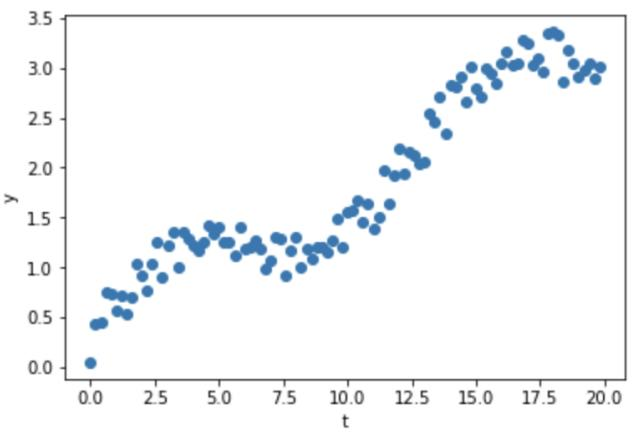
\includegraphics[keepaspectratio,
                   width=.5\paperwidth]{ts_example.jpg}
  \end{center}
\end{frame}


\begin{frame}
  \frametitle{Типы зависимостей}

  \begin{center}
    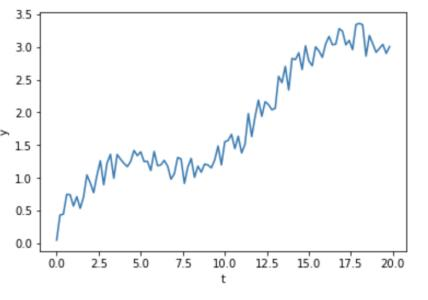
\includegraphics[keepaspectratio,
                   width=.5\paperwidth]{raw_signal.jpg}
  \end{center}

  \begin{tabular}{cccc}
    тренд \hfill & сезонность & стороннее влияние & остальной сигнал \\
    \hspace{-1.2cm}
    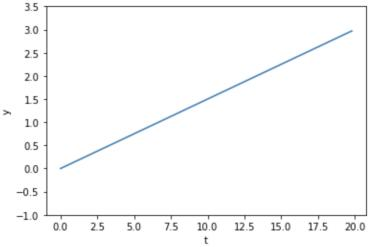
\includegraphics[keepaspectratio,
                   width=.2\paperwidth]{trend.jpg}
    &
    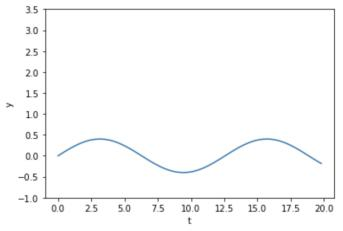
\includegraphics[keepaspectratio,
                   width=.2\paperwidth]{season.jpg}
    &
    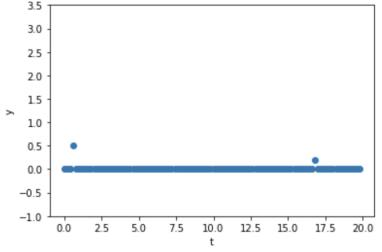
\includegraphics[keepaspectratio,
                   width=.2\paperwidth]{site_impact.jpg}
    &
    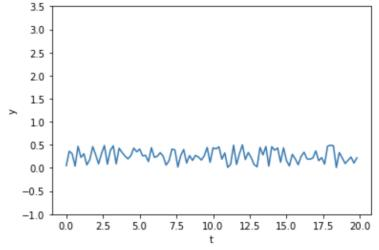
\includegraphics[keepaspectratio,
                   width=.2\paperwidth]{other_signal.jpg}
  \end{tabular}
\end{frame}


\begin{frame}
  \begin{question}
    Какой сильный baseline всегда есть в моделировании временных рядов?
  \end{question}
  \pause
  \vspace{2cm}
  \begin{block}{Замечание}
  Кроме непосредственно следующего значения ряда нужно оценивать предсказательный интервал прогноза (prediction interval)
\end{block}
\end{frame}


\begin{frame}
  \frametitle{Подходы}

  \begin{itemize}
    \item модели экспоненциального сглаживания
    \item ARMA — autoregressive moving average
    \item TBATS — Trigonometric, Box-Cox transformation, ARMA, Trend, Seasonality
    \item нейронные сети, конечно
    \item {\bf ARIMA}
    \item {\bf Prophet}
  \end{itemize}
\end{frame}

\begin{frame}
  \frametitle{ARIMA}

  {\bf Стационарные временные ряды}

  \vspace{1cm}
  Строгая стационарность

  $ p(y_t, y_{t+1}, \dots , y_T) = p(y_{t+\tau}, y_{t+1+\tau},\dots, y_{T+\tau}) $

  \vspace{1cm}
  Стационарность в смысле ковариации (weak or wide-sense stationarity):
  \begin{align*}
    E(y_1) &= E(y_2) = \dots = \text{const} \\
    \text{Var}(y_1) &= \text{Var}(y_2) = \dots = \text{const} \\
      \text{Cov}(y_t, y_{t+k}) &= \text{Cov}(y_{t+\tau}, y_{t+k+\tau}) = \gamma_k
  \end{align*}
\end{frame}


\begin{frame}
  \frametitle{Пример: стационарный временной ряд}

  Белый шум $\varepsilon_t$

  $$ E(\varepsilon_t) = 0,\ \text{Var}(\varepsilon_t) = \sigma^2$$

  $$ \text{Cov}(\varepsilon_t, \varepsilon_{t+k}) = 0 $$

  \begin{center}
    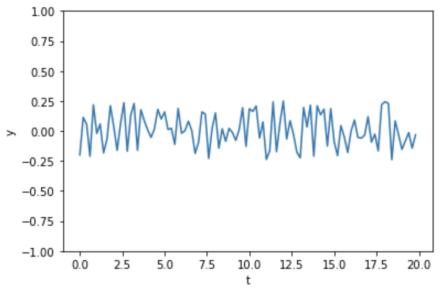
\includegraphics[keepaspectratio,
                     width=.7\paperwidth]{stationary.jpg}
  \end{center}
\end{frame}


\begin{frame}
  \frametitle{Пример: нестационарный временной ряд с линейным трендом}

  Процесс с детерминистическим трендом

  $$ y_t = 5 + 0.1t + \varepsilon_t $$

  \begin{center}
    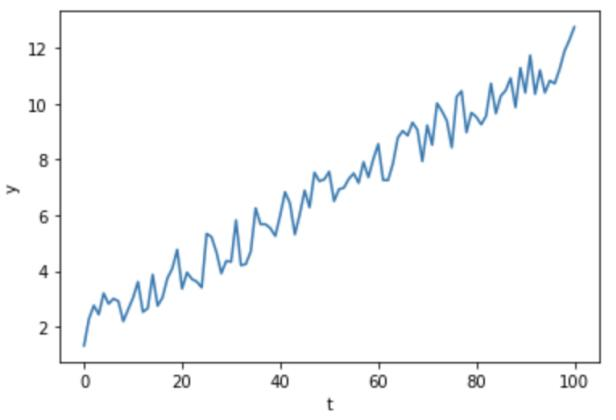
\includegraphics[keepaspectratio,
                     width=.7\paperwidth]{lin_unstationary.jpg}
  \end{center}
 \end{frame}


\begin{frame}
  \frametitle{Пример: нестационарный временной ряд — случайное блуждание}

  Процесс с детерминистическим трендом

  $$ y_t = 1 + y_{t-1} + \varepsilon_t $$

  \begin{center}
    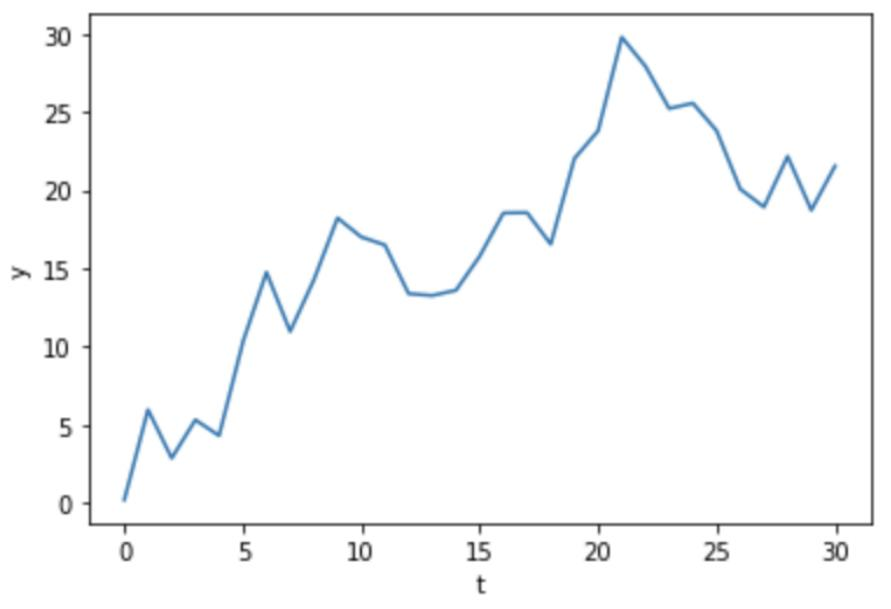
\includegraphics[keepaspectratio,
                     width=.7\paperwidth]{random_unst.jpg}
  \end{center}
\end{frame}


\begin{frame}
  \frametitle{Стационарные временные ряды. Модель скользящего среднего: MA(q)}

  $$ y_t = \mu + \varepsilon_t + a_1\varepsilon_{t-1} + \dots + a_q\varepsilon_{t-q} $$

  $$ y_t = 1 + \varepsilon_t + 0.2\varepsilon_{t-1} + 0.3\varepsilon_{t-2} + 0.1\varepsilon_{t-3} $$

  \begin{center}
    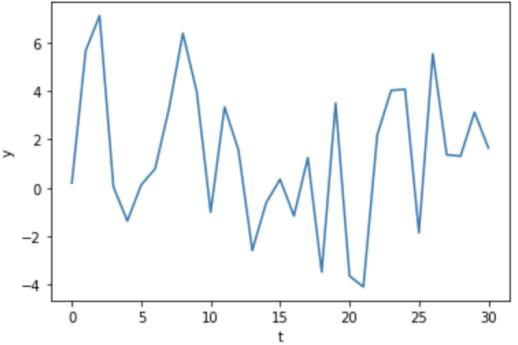
\includegraphics[keepaspectratio,
                     width=.6\paperwidth]{mean_average_model.jpg}
  \end{center}
\end{frame}


\begin{frame}
  \frametitle{Модель скользящего среднего: MA(q) — посчитаем статистики}

  $y_t = 1 + \varepsilon_t + 0.2\varepsilon_{t-1} + 0.3\varepsilon_{t-2}, \quad \varepsilon \sim N(0, \sigma^2) $

  \begin{align*}
    \text{Var}(y_t) &= \text{Var}(1 + \varepsilon_t + 0.2\varepsilon_{t-1} + 0.3\varepsilon_{t-2}) = \\
      &= (1^2 + 0.2^2 + 0.3^2) \sigma^2 = 1.13\sigma^2 \\
    \gamma_1 &= \text{Cov}(y_t, y_{t-1}) = \\
     &=  \text{Cov}(1 + \varepsilon_t + 0.2\varepsilon_{t-1} + 0.3\varepsilon_{t-2},\\
     & 1 + \varepsilon_{t-1} + 0.2\varepsilon_{t-2} + 0.3\varepsilon_{t-3}) = \\
     &= \text{\{с одинаковыми индексами не нулевые\}} = \\
     &= (0.2 + 0.3*0.2) \sigma^2 = 0.26\sigma^2 \\
    \gamma_2 &= 0.3\sigma^2 \\
    \gamma_3 &= 0
  \end{align*}

  Запомним, что с $\gamma_3$ все нулевые!
\end{frame}


\begin{frame}
   \begin{block}{Стационарные временные ряды. Автокорреляция}
     $$ \text{Corr}(y_t, y_{t-k}) = \frac{\text{Cov}(y_t, y_{t-k})}{\sqrt{\text{Var}(y_t)\text{Var}(y_{t-k})}} = \frac{\gamma_k}{\gamma_0}$$
   \end{block}

\end{frame}


\begin{frame}{Кореллограммы}

  \begin{center}
    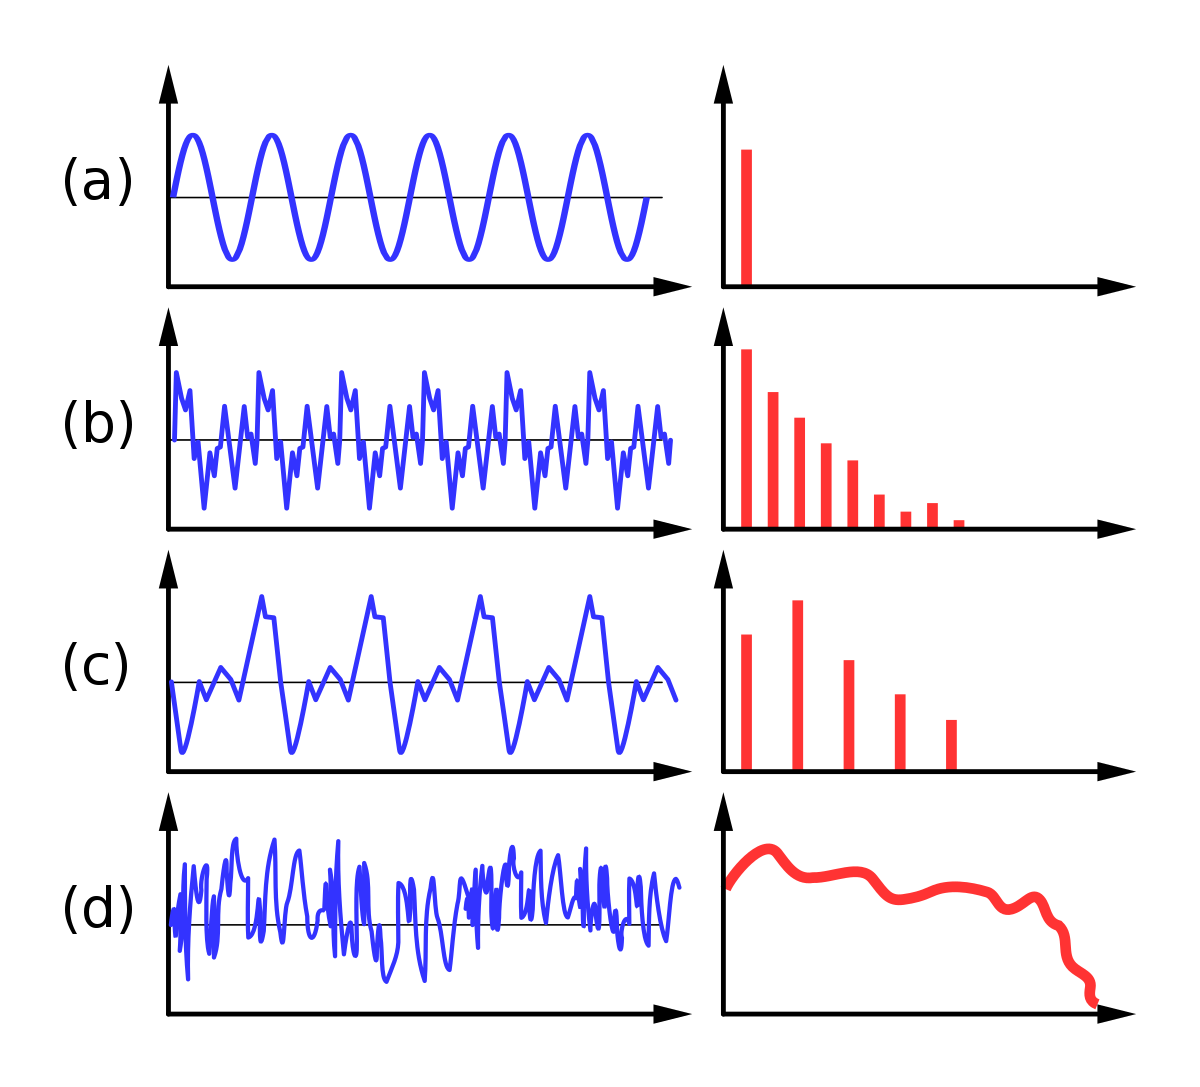
\includegraphics[keepaspectratio,
                     width=.75\paperwidth]{correlograms.png}
  \end{center}

\end{frame}


\begin{frame}
  \begin{block}{Частная автокорреляция}
    \begin{align*}
      \text{PartCorr}(y_t, y_{t-k}) = \text{Corr}(y_t - \text{Proj}(y_t|y_{t-1}\dots y_{t-k+1}), \\
      y_{t-k} - \text{Proj}(y_{t-k}|y_{t-1}\dots y_{t-k+1})
    \end{align*}
  \end{block}

 где $\text{Proj}(z|y_{t-1}\dots y_{t-k+1})$ — ортогональная проекция $z$ на линейное подпространство Гильбертова пространства, построенное на ${y_{t-1},\dots ,y_{t-k+1}}$

 \begin{center}
   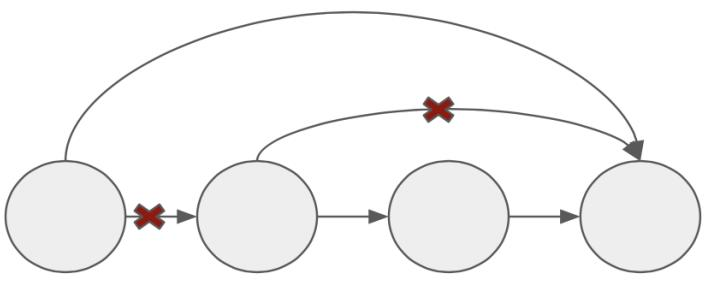
\includegraphics[keepaspectratio,
                    width=.4\paperwidth]{partial_autocorr.jpg}
 \end{center}
\end{frame}


\begin{frame}
  \frametitle{Стационарные временные ряды. Процесс авторегрессии}

  $$ y_t = c + b_1y_{t-1} + b_2y_{t-2} + \dots + b_py_{t-p} + \varepsilon_t $$

  Авторегрессия:

  $$ y_t = 1 + 0.25y_{t-1} + \varepsilon_t $$

  \begin{center}
    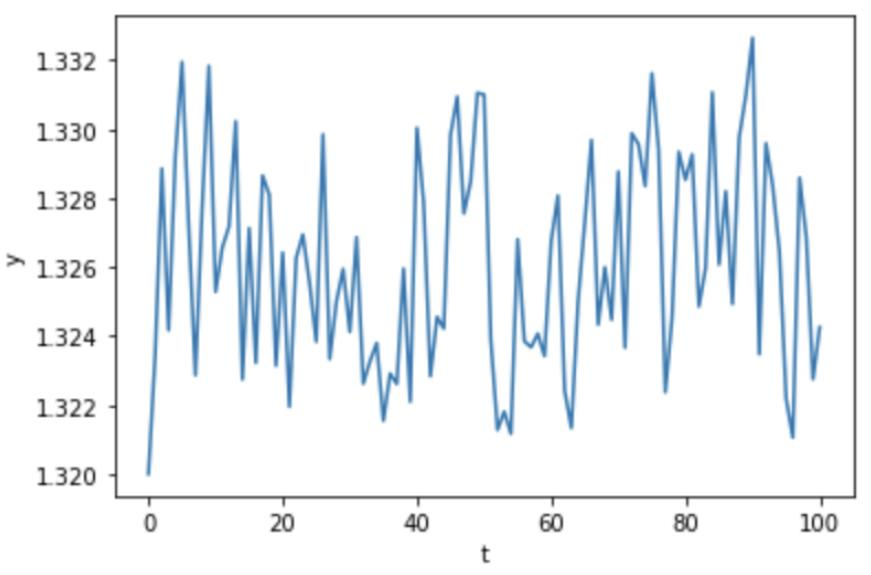
\includegraphics[keepaspectratio,
                     width=.6\paperwidth]{autoregression.jpg}
  \end{center}
\end{frame}


\begin{frame}
  \begin{question}
    Как определить по временному ряду стационарный ли он?
  \end{question}
  \pause
  \begin{block}{Проверка на стационарность}
    $y_t = 1 + y_{t-1} + \varepsilon_t$ — нестационарный

    $y_t = 1 + 0.25y_{t-1} + \varepsilon_t$ — стационарный
  \end{block}
\end{frame}


\begin{frame}
  \frametitle{Оператор лага. Характеристический многочлен}

  Пусть $L$ — оператор лага, то есть $y_{t-1} = Ly_t$

  тогда уравнение авторегрессии можно переписать в виде

  $y_t = c + b_1Ly_t + b_2L^2y_t + \dots + b_pL^py_t + \varepsilon_t$

  или

  $(1 - b_1L - b_2L^2 - \dots - b_pL^p)y_t = c + \varepsilon_t$

  \begin{block}{Теорема}
    Если корни характеристического многочлена $(1 - b_1L - b_2L^2 - \dots - b_pL^p)$ по модулю больше 1, то процесс стационарен в смысле ковариации
  \end{block}

  \noindent\rule{8cm}{0.4pt}

  {\it Shumway, Robert; Stoffer, David.} (2010) Time series analysis and its applications: with R examples (3rd ed.). Springer. ISBN 144197864X. (p. 88-90)
\end{frame}


\begin{frame}
  \frametitle{Получение прогноза из формулы процесса}

  $$ y_t = c + b_1y_{t-1} + b_2y_{t-2} + \dots + b_py_{t-p} + \varepsilon_t $$

  $\forall i \leq t$ известны $y_i$

  $$ y_{t+1}, y_{t+2}, \dots = ? $$

  \vspace{1cm}
  Ответ:

  $$ \hat y_{t+1} = E (y_{t+1}| y_t, \dots, y_{t-p}) $$

  $+$ оценка дисперсии в качестве предсказательного интервала
\end{frame}


\begin{frame}
  \frametitle{Получение прогноза из формулы процесса. Пример}

  $$ y_t = 1 + 0.25y_{t-1} + \varepsilon_t, \varepsilon_t \sim N(0, 0.2) $$

  Пусть $y_t = 2$

  \begin{align*}
     \hat y_{t+1} = E(y_{t+1} &| y_{t}) = E(1 + 0.25y_{t} + \varepsilon_{t+1}) = 1 + 0.25*2 + 0 = 1.5 \\
     \text{Var}(y_{t+1} | y_{t}) &= \text{Var}(1 + 0.25y_{t} + \varepsilon_{t+1}) = \text{Var}(\varepsilon_{t+1}) = 0.2
  \end{align*}

  \begin{align*}
     \hat y_{t+2} = E(y_{t+2} &| y_{t+1}) = E(1 + 0.25y_{t+1} + \varepsilon_{t+2}) = 1 + 0.25 * 1.5 = 1.375 \\
     \text{Var}(y_{t+2}) &= \text{Var}(1 + 0.25y_{t+1} + \varepsilon_{t+2}) = 0.25^2 * 0.2 + 0.2 = 0.2125
     \end{align*}
\end{frame}


\begin{frame}
  \frametitle{Процесс ARMA(p, q)}

  $ y_t = b_1y_{t-1} + b_2y_{t-2} + \dots + b_py_{t-p} + \varepsilon_t + c + \varepsilon_t + a_1\varepsilon_{t-1} + \dots + a_q\varepsilon_{t-q} $
  \pause
  \vspace{1cm}
  \begin{question}
    Как определить $p$ и $q$?
  \end{question}
\end{frame}


\begin{frame}
  \frametitle{Cтационарные ряды и процесс ARMA(p, q)}

  \begin{block}{Теорема Волда}
   Теорема из математической статистики, согласно которой каждый слабо стационарный временной ряд можно представить в виде скользящего среднего бесконечного порядка $\mathrm{MA}(\infty)$.
  \end{block}

  Такое представление называют скользящим средним для временных рядов.

  \vspace{1cm}
  $\mathrm{ARMA}(p, q)$ приближает $\mathrm{MA}(\infty)$ с любой необходимой точностью.
\end{frame}


\begin{frame}
  \frametitle{Подбор коэффициентов $p$ и $q$ на практике}

  Начальные приближения $p$ и $q$ выбираем следующим образом:

  $q$ — смотрим на график оценок автокорреляций (ACF)

  $$ \hat{Corr}(y_t, y_{t-k}) = \frac{\sum\limits_{t=k+1}^T (y_t - \overline{y})(y_{t-k} - \overline{y}) }{\sum\limits_{t=1}^T (y_t - \overline{y})^2} $$

  \vspace{1cm}
  $p$ — смотрим на график оценок частных автокорреляций (PACF), последовательно обучая авторегрессии

  $$ \hat y = . + .y_{t-1} + .y_{t-2} + \dots + \phi_k y_{t-k} + \nu_t $$

  Проверяем значимость, например, с помощью t-критерия.
\end{frame}


\begin{frame}
  \frametitle{Оценка качества моделей}

  \begin{block}{Критерий Акаике}
    (чем меньше, тем лучше модель)

    $$ \text{AIC} = 2k - 2log(L)$$

    $k$ — количество параметров

    $L$ — правдоподобие выборки
  \end{block}
\end{frame}


\begin{frame}
  \frametitle{Приведение ряда к стационарному. Удаление тренда}

  {\bf Удаление тренда} — дифференцирование $y^\prime_t = y_t - y_{t-1}$ и сезонное дифференцирование $y^{\prime\prime}_t = y_t - y_{t-12}$

  \vspace{0.5cm}
  Таким образом приходим к модели {\bf ARIMA(p,d,q)}, где $d$ — число дифференцирований

  \vspace{0.5cm}
  \begin{tabular}{cc}
    \hspace{-1cm}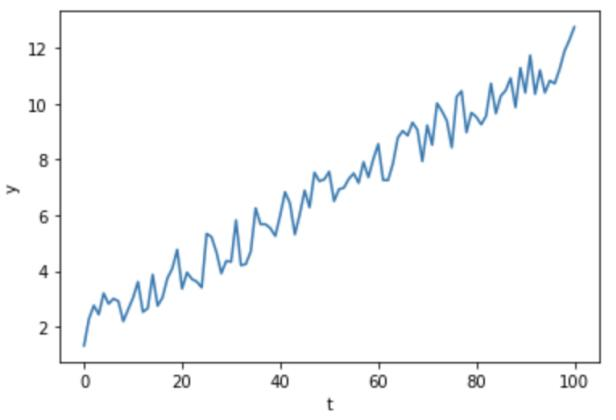
\includegraphics[keepaspectratio,
                     width=.45\paperwidth]{lin_unstationary.jpg}
    &
    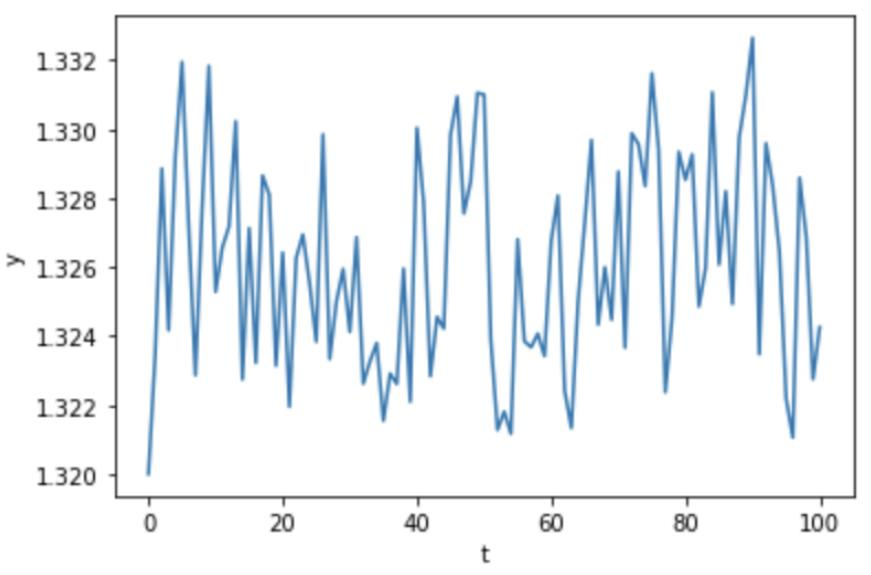
\includegraphics[keepaspectratio,
                     width=.45\paperwidth]{autoregression.jpg}
  \end{tabular}
  \begin{center}
  \end{center}
\end{frame}


\begin{frame}
  \frametitle{Приведение ряда к стационарному. Гетероскедастичность}

  Преобразование Бокса-Кокса:

  $$ y_t^n =
    \begin{cases}
    \ln y_t,  \lambda = 0 \\
    \frac{(y_t^\lambda - 1)}{\lambda}, \lambda \neq 0
    \end{cases}
  $$

  \vspace{0.5cm}
  \begin{center}
    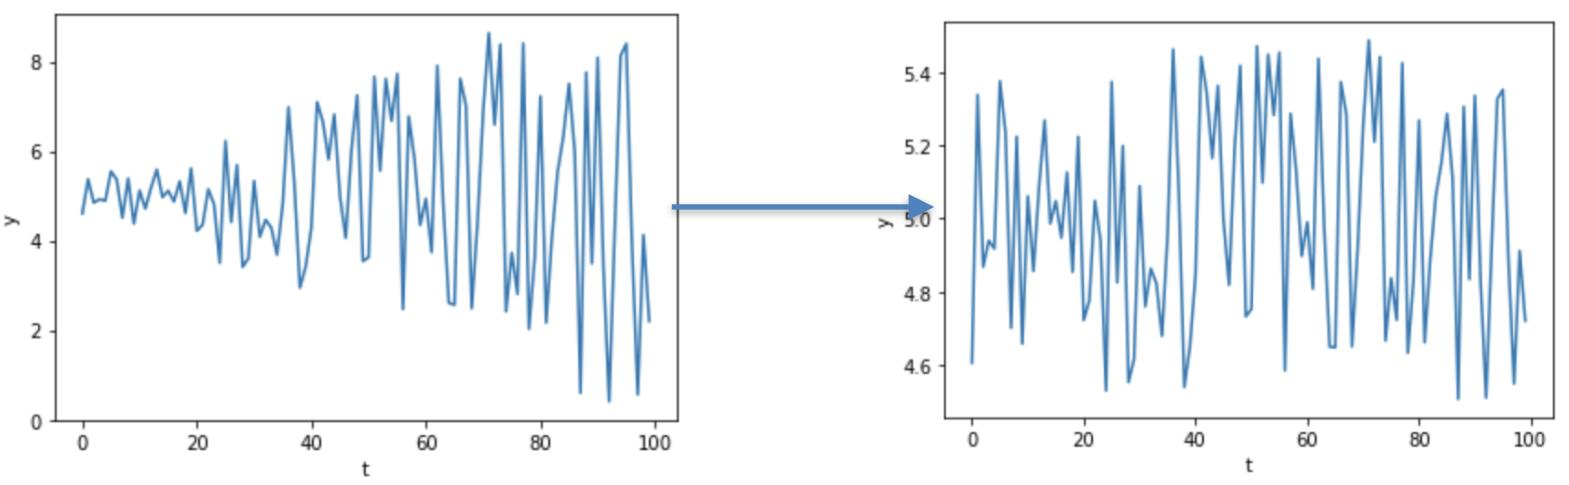
\includegraphics[keepaspectratio,
                     width=.85\paperwidth]{heteroscedasticity.jpg}
  \end{center}

\end{frame}


\begin{frame}
  \frametitle{План действий при использовании ARIMA}
  \begin{enumerate}
    \item Смотрим на данные
    \item При необходимости используем преобразование Бокса-Кокса
    \item Дифференцируем ряд, пока он не станет стационарным (проверяем, например, с помощью теста Дики-Фуллера)
    \item строим графики ACF и PACF, подбираем $p, q$ в модели
    \item оцениваем построенные модели с помощью AIC
    \item проверяем остатки на наличие автокорреляции (например, с помощью Q-критерия Льюнга-Бокса)
  \end{enumerate}
\end{frame}


\begin{frame}
  \frametitle{Типы зависимостей}

  \begin{center}
    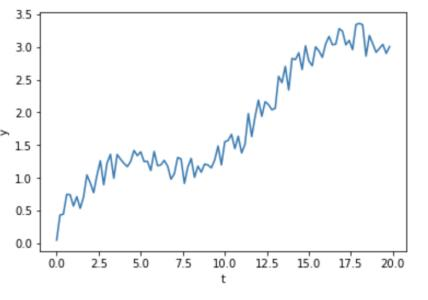
\includegraphics[keepaspectratio,
                   width=.5\paperwidth]{raw_signal.jpg}
  \end{center}


  \begin{tabular}{cccc}
    тренд \hfill & сезонность & стороннее влияние & остальной сигнал \\
    \hspace{-1.2cm}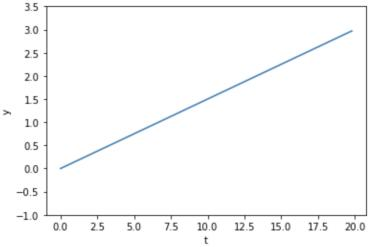
\includegraphics[keepaspectratio,
                   width=.2\paperwidth]{trend.jpg}
    &
    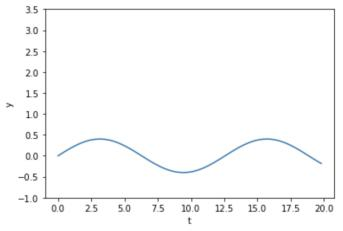
\includegraphics[keepaspectratio,
                   width=.2\paperwidth]{season.jpg}
    &
    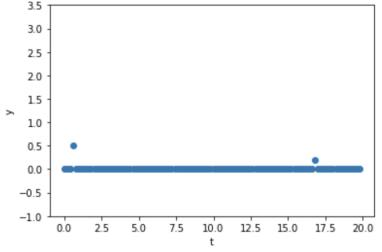
\includegraphics[keepaspectratio,
                   width=.2\paperwidth]{site_impact.jpg}
    &
    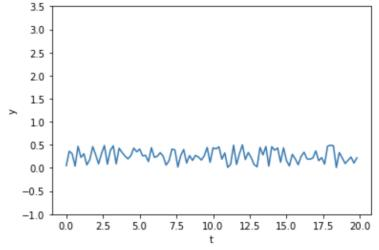
\includegraphics[keepaspectratio,
                   width=.2\paperwidth]{other_signal.jpg}
  \end{tabular}
\end{frame}


\begin{frame}
  \frametitle{Prophet}

  $$ y(t) = g(t) + s(t) + h(t) + \varepsilon_t $$

  Здесь

  $g(t)$ — функция тренда

  $s(t)$ — функция сезонности

  $h(t)$ — функция различных событий

  $\varepsilon_t$ — неучтённое влияние
\end{frame}


\begin{frame}
  \frametitle{Prophet. Тренд}

  Виды трендов:
  \begin{itemize}
    \item линейный $g(t) = kt + m$
    \item нелинейный затухающий $g(t) = \frac{C}{1 + \exp(-k(t-m))}$
  \end{itemize}

  \vspace{1cm}
  Для соц.сетей (Facebook, ВКонтакте) актуально, например, прогнозировать количество их пользователей в разных регионах, поэтому такой вариант нелинейного затухающего $g(t)$
\end{frame}


\begin{frame}
  \frametitle{Prophet. Учёт точек изменения тренда}

  \begin{center}
    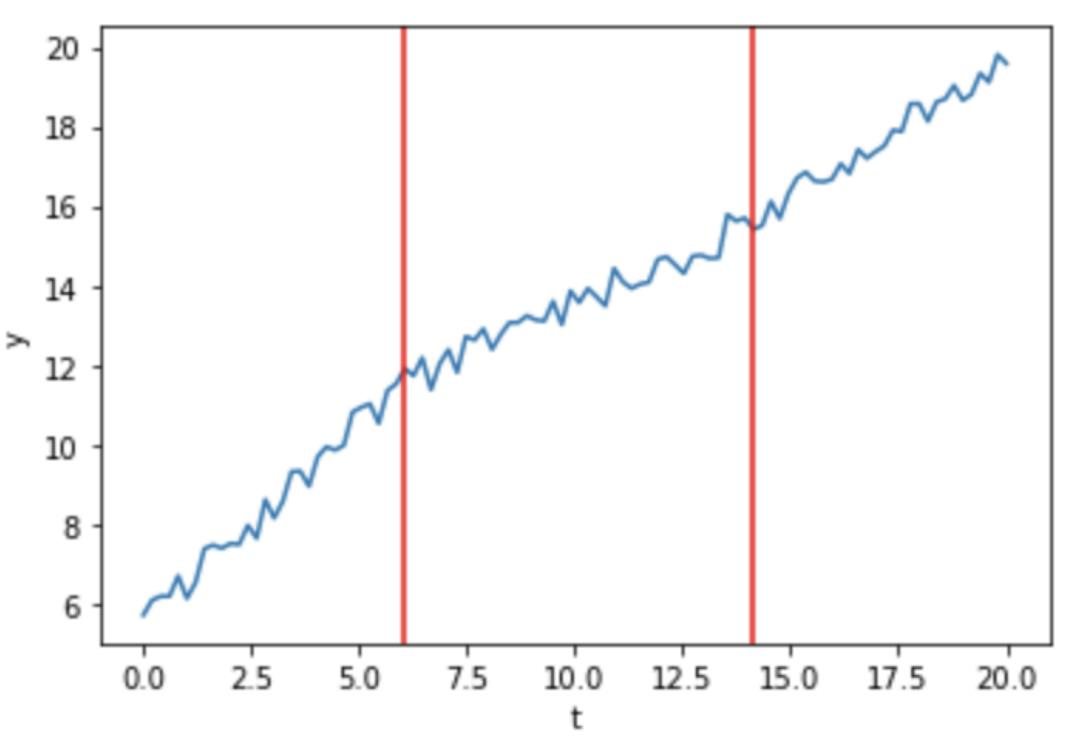
\includegraphics[keepaspectratio,
                   width=.6\paperwidth]{trend_change.jpg}
  \end{center}
\end{frame}


\begin{frame}
  \frametitle{Prophet. Учёт точек изменения тренда}

  Предполагаем наличие $S$ точек смены тренда $s_j, j = 1, \dots, S$

  определяем вектор изменений $\delta \in R^S$

  и вычисляем значение $k$ в момент времени $t$ по формуле

  $$ k + \sum\limits_{j:t > s_j} \delta_j $$

  также это можно задать в виде перемножения матрицы эффекта $\delta$ и матрицы достижения следующей точки изменения тренда

  $$ a_j(t) =
    \begin{cases}
    1, t \geq s_j \\
    0, \text{иначе}
    \end{cases}
  $$

  Адаптируем сдвиги, избегая разрывов: $$\gamma_j = \left(s_j - m - \sum\limits_{p < j}\gamma_p \right) \left(1 - \frac{k+\sum\limits_{p < j}\delta_p}{k+\sum\limits_{p \leq j}\delta_p} \right)$$

\end{frame}


\begin{frame}
  Получаем итоговую формулу
  $$ g(t) =
  \frac{С(t)}
  {1 + \exp(
      -(k + \boldsymbol{a}(t)^T\boldsymbol{\delta})
       (t - (m + \boldsymbol{a}(t)^T\boldsymbol{\gamma}))
      )
  }
  $$

  Или для линейного тренда
  $$ g(t) =
      (k + \boldsymbol{a}(t)^T\boldsymbol{\delta})t
      +(m + \boldsymbol{a}(t)^T\boldsymbol{\gamma})
  $$
\end{frame}


\begin{frame}
  \frametitle{Prophet. Автоматический отбор точек}

  $$ \delta_j \sim \text{Laplace}(0, \tau) $$

  (эквивалентно $L_1$-регуляризации для линейной модели)
\end{frame}


\begin{frame}
  \frametitle{Prophet. Сезонность}

  \begin{center}
    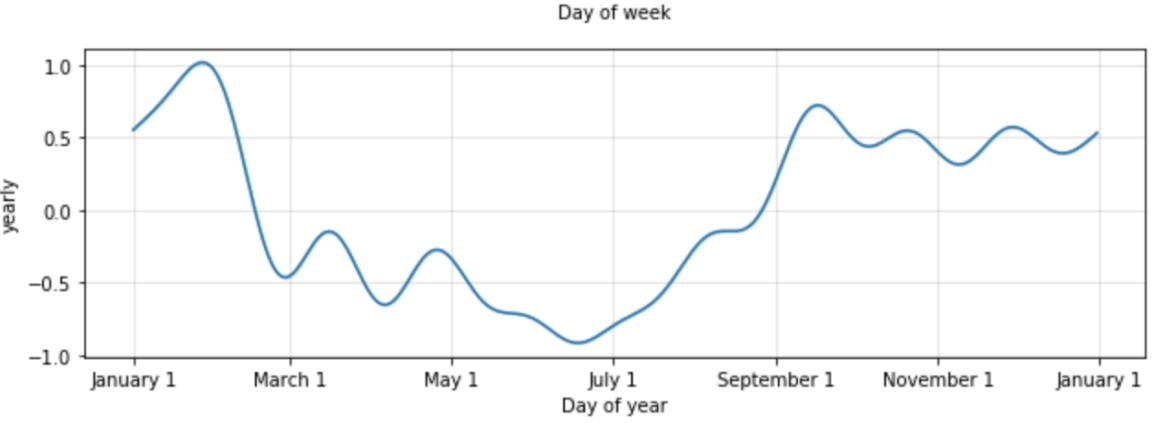
\includegraphics[keepaspectratio,
                   width=.8\paperwidth]{seasons.jpg}
  \end{center}

\end{frame}


\begin{frame}
  \frametitle{Моделируем рядами Фурье}

  \begin{align*}
    s(t) &= \sum\limits_{n=1}^N \left(a_n \cos\left(\frac{2\pi nt}{P}\right) + b_n \sin\left(\frac{2\pi nt}{P} \right) \right) \\
    \beta &= [a_1, b_1, \dots, a_N, b_N], \text{ априори } \beta \sim N(0, \sigma^2)\\
    X(t) &= \left[ \cos\left(\frac{2\pi(1)t}{365.25}\right), \dots, \sin\left(\frac{2\pi(10)t}{365.25}\right) \right]
  \end{align*}

  \vspace{1cm}
  \begin{center}
    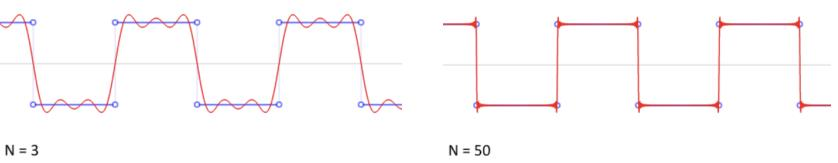
\includegraphics[keepaspectratio,
                   width=.8\paperwidth]{fourie.jpg}
  \end{center}

\end{frame}


\begin{frame}
  \frametitle{Prophet. События}

  \begin{align*}
    Z(t) &= [\mathbb{I}(t \in D_1), \dots, \mathbb{I}(t \in D_L)]\\
         &\omega\ - \text{ величины влияния праздников } \\
       h(t) &= Z(t)^T \omega
  \end{align*}

\end{frame}


\begin{frame}
  \frametitle{Возможные регрессионные признаки}

  \begin{itemize}
    \item гармоники по длинным периодам сезонности
    \item индикаторы номера периода в коротких сезонностях
    \item индикаторы праздников
    \item индикаторы пред- и постпраздничных дней
    \item тренды (линейный, квадратичный и т.п.)
    \item скользящие средние ряда
    \item ...
  \end{itemize}

\end{frame}


\begin{frame}
  \frametitle{Как ещё можно моделировать временные ряды}
  \begin{itemize}
    \item статистики за прошлые периоды и знакомый бустинг
    \item нейронные сети, как рекуррентные, так и свёрточные
    \item стекинг моделей
  \end{itemize}
\end{frame}


\begin{frame}
  \frametitle{Резюме}
  \begin{itemize}
    \item временной ряд — зависимые наблюдения с одинаковым шагом по времени
    \item стационарные и нестационарные временные ряды
    \item ARIMA — авторегрессия с дифференцированием и моделью скользящего среднего
    \item Prophet — популярная библиотека моделирования временных рядов
  \end{itemize}
  \pause
  Что ещё можно посмотреть?
  \begin{itemize}
    \item \href{https://www.youtube.com/watch?v=u433nrxdf5k}{Лекция Евгения Рябенко} о прогнозировании временных рядов
    \item \href{https://facebook.github.io/prophet/}{https://facebook.github.io/prophet/}
    \item Книга Hyndman «Forecasting: Priciples And Practice» — библия прогнозирования временных рядов
  \end{itemize}
\end{frame}

\end{document}
